\RequirePackage{fix-cm}
\documentclass[twocolumn]{svjour3}          % twocolumn
\journalname{Behavior Research Methods}


%\documentclass[jou,apacite]{apa6}
%\shorttitle{Online behavioral research with psiTurk}
%
%\twoauthors{Author One}{Author Two}
%\twoaffiliations{Institute of Psychology}{Freud's Institute}
%
%\abstract{psiTurk is really great and you should use it.}
%
%\rightheader{Online behavioral research with psiTurk}
%\leftheader{Online behavioral research with psiTurk}

\usepackage{listings}
\usepackage{color}
\usepackage{graphicx}
\usepackage{soul}
\usepackage{natbib}


\definecolor{dkgreen}{rgb}{0,0.6,0}
\definecolor{gray}{rgb}{0.5,0.5,0.5}
\definecolor{mauve}{rgb}{0.58,0,0.82}

\renewcommand{\labelitemi}{$\bullet$}
\renewcommand{\labelitemii}{$\cdot$}

\lstset{frame=tb,
  %language=Java,
  aboveskip=5mm,
  belowskip=5mm,
  showstringspaces=false,
  columns=flexible,
  basicstyle={\ttfamily},
  numbers=none,
  numberstyle=\tiny\color{gray},
  keywordstyle=\color{blue},
  commentstyle=\color{dkgreen},
  stringstyle=\color{mauve},
  frame=none,
  breaklines=true,
  breakatwhitespace=true
  tabsize=3
}

% commands for formatting psiTurk and psiturk.js, for consistency
\newcommand{\psiturk}[0]{\textsf{psiTurk}}
\newcommand{\psiturkjs}[0]{\emph{psiturk.js}}

\begin{document}

\title{\psiturk{}: An open-source framework for conducting replicable behavioral experiments online}

% i set the authorship order based on github contributions
\author{Todd M. Gureckis$^1$ \and
	Jay Martin$^{1,2}$ \and
	John McDonnell$^3$ \and
	Alexander S. Rich$^1$ \and
	Doug Markant$^4$  \and
	Anna Coenen$^1$ \and
	David Halpern$^1$ \and
	Jessica B. Hamrick$^5$ \and
	Patricia Chan$^1$
}


%\authorrunning{Short form of author list} % if too long for running head

\institute{
$^1$Department of Psychology, New York University\\
$^2$Stitch Fix, Inc.\\
$^3$Square, Inc.\\
$^4$Center for Adaptive Rationality, Max Planck Institute for Human
Development\\
$^5$Department of Psychology, University of California at Berkeley\\
\\
\psiturk{} was primarily written by the listed authors at the time the
first draft of this paper was constructed (version 2.0.0).  However, many people 
continually contribute to \psiturk{}'s evolving code base and
documentation via GitHub.  Illustrations by Kylan Larson (\textsf{http://kylanlarson.com}).
\\
\\
Please address correspondence concerning this paper to:\\
	Todd M. Gureckis \at
	New York University\\
	Department of Psychology \\
        \email{authors@psiturk.org}
}

\date{Received: 1/4/2014 date}

\maketitle

\begin{abstract}
Online data collection has begun to revolutionize the behavioral sciences.  
However, conducting carefully controlled behavioral experiments online introduces a number of new
of technical and scientific challenges.  The project described in this paper, \textsf{psiTurk}, is 
an open-source platform which helps researchers develop experiment designs which can be
conducted over the Internet.  The tool primarily interfaces with Amazon's Mechanical Turk, 
a popular crowd-sourcing labor market.  This paper describes the basic architecture of the system 
and introduces new users to the overall goals of the system.  \textsf{psiTurk} aims to reduce
the technical hurdles for researchers developing online experiments 
while improving the transparency and collaborative nature of the behavioral sciences.
\keywords{Online experiments \and Open science \and Amazon Mechanical Turk \and Internet Experiments \and psiTurk}
\end{abstract}

\tolerance=5000

\section{Introduction}


The ability to collect behavioral data from a large group of individuals
anonymously over the Internet has transformed the behavioral and social
sciences.  In addition to large scale experiments such as those
conducted by websites such as Facebook or 
Twitter~\citep[e.g.,][]{Chen:2013pb,Kramer:2014dq,Wu:2011sp}, many researchers
use online data collection to deploy ``traditional'' experimental psychology
tasks.  The benefit of the online versions of traditional behavioral experiments include 
faster data collection and access to a potentially more diverse pool of participants. 
At the same time, conducting experiments online introduces a number of new 
technical and scientific challenges that must be addressed.

The project described in this paper, \psiturk{}, is an open-source project that aims to address many of the technical challenges
involved in deploying psychology experiments online.
It facilitates the creation, deployment, sharing, and replication of web-based experiments.
Study participants can be recruited via Amazon 
Mechanical Turk (AMT), which is currently the most popular platform for running 
paid human experiments online.

\begin{figure*}[tp]
\centering
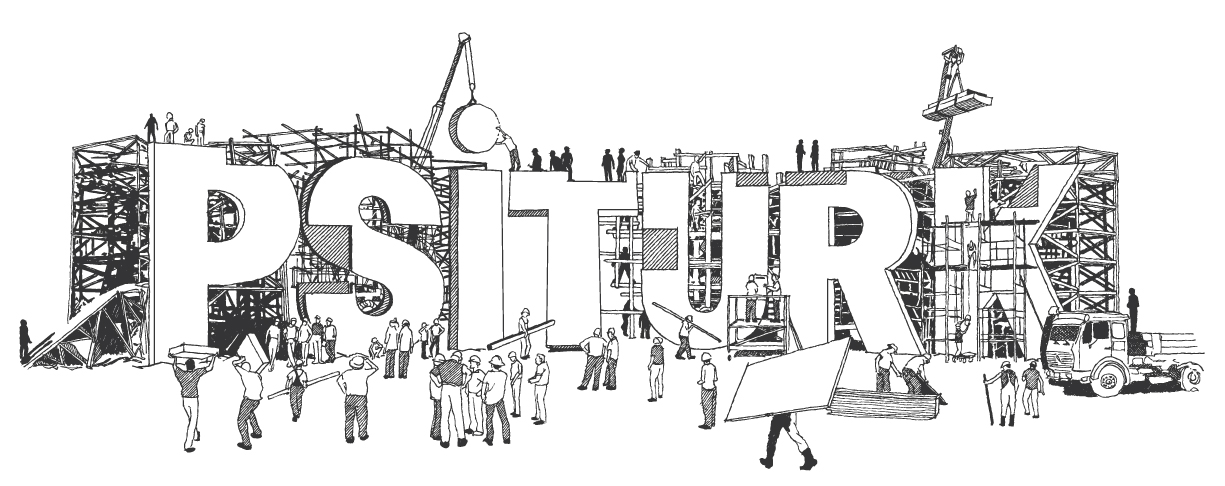
\includegraphics[scale=.30]{figures/psiturk_logo.jpg}
\caption{The \psiturk{} project is hosted on GitHub 
(\textsf{https://github.com/NYUCCL/psiTurk}) and at its main webpage (\textsf{https://psiturk.org}). 
The commissioned logo reflects the community-built orientation of the project.  A 
core philosophy is that better scientific software can be developed 
with more diverse input from many programmers~\citep{Raymond:1999zt}.}
\label{fig:logo}
\end{figure*}

To briefly summarize, \psiturk{} provides a python-based web server and associated javascipt library for conducting 
experiments on the web, saving experimental data to a database, and restricting the 
participant pool according to the experimenter's needs (e.g., to prevent from repeating a study). 
It also provides a command-line interface with AMT to 
create and test new projects as well as to manage and pay participants. Finally, in 
the spirit of the recent ``open science'' movement \citep{Collaboration:2012vf},
it provides  an open-source Experiment Exchange for sharing experiments 
that can be easily replicated and extended by other researchers.  The code for 
\psiturk{} is open source, hosted publicly at
\textsf{https://github.com/NYUCCL/psiTurk}, and interested researchers can easily 
contribute to improvements and bug fixes (see Figure~\ref{fig:logo}).

The principal goal of \psiturk{} is to handle common technical 
challenges so that researchers can focus on the development and replication
of online experiments.  In this paper, we present a high-level overview of the 
\psiturk{} framework and its advantages for running web-based experiments.
In supplement to this overview, \psiturk{} provides a large and continually
evolving set of documentation hosted online (\textsf{https://psiturk.org/docs}).
We begin with an overview of the issues involved in online 
behavioral research,  the AMT platform, and the specific challenges that \psiturk{} is designed to 
address.  We then  step through the core functionality of \psiturk{} and 
describe its role from the point of view of both the experimenter and the participant.  Finally, we
consider some future directions for \psiturk{} and online experimentation in 
general.



\section{The challenges of web-based experimental behavioral research}

\begin{figure*}[tp]
\centering
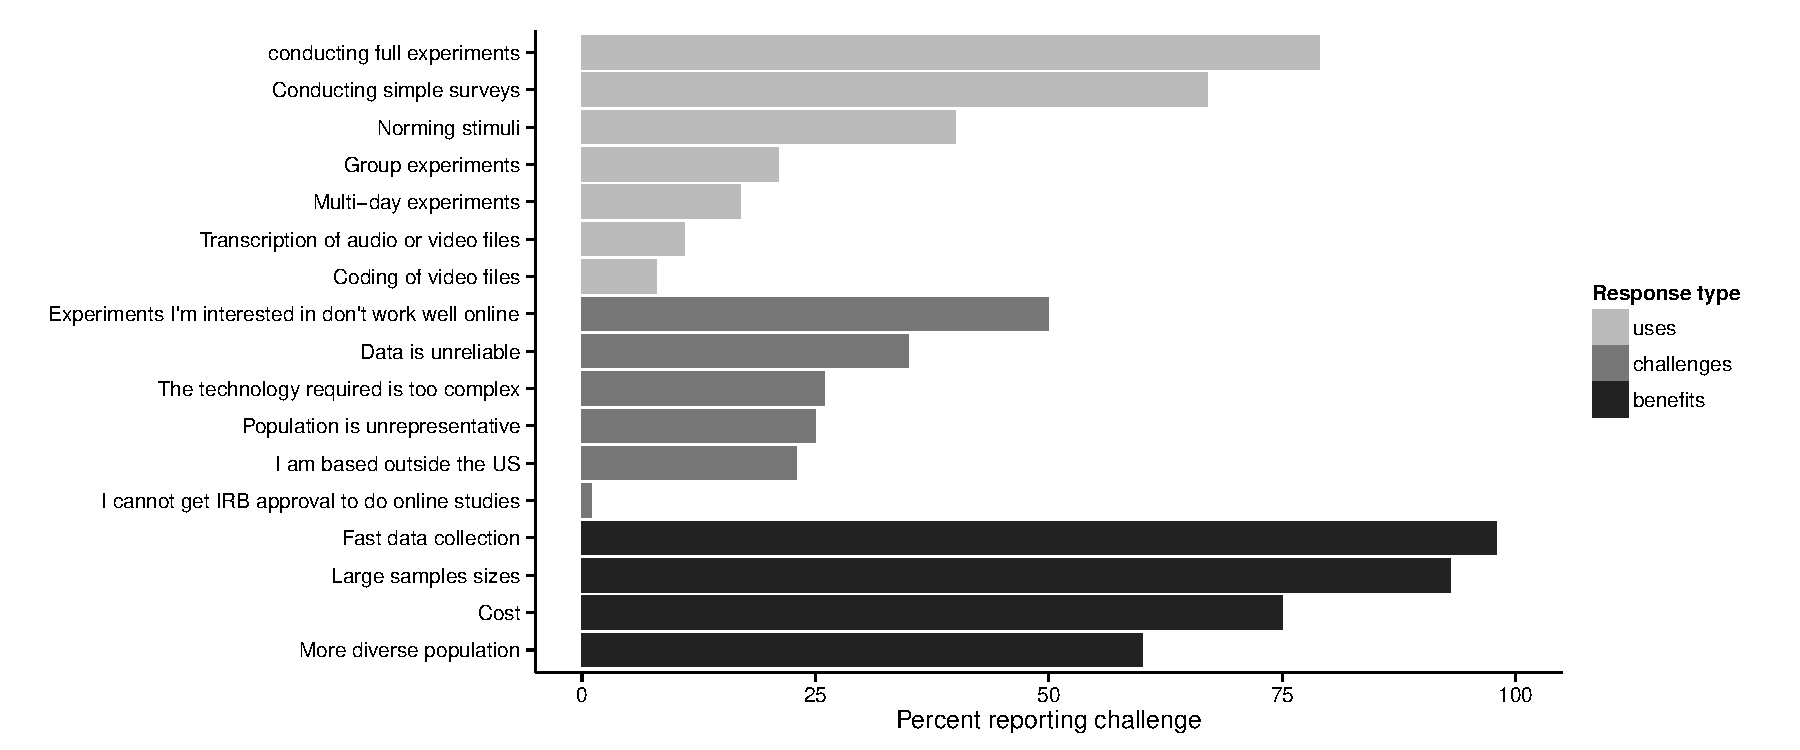
\includegraphics[width=\textwidth]{figures/combinedquestions2.pdf}
\caption{Reported uses, challenges, and benefits of online data collection as surveyed
by 201 behavioral researchers.}
\label{fig:survey}
\end{figure*}

It is easy to see why online experiments are an attractive option for behavioral 
scientists.  Compared to traditional methods of experimentation in the laboratory,
they allow researchers to collect large data sets in a fraction of the time and at 
much lower cost (in terms of time, employment of research assistants, and typical 
compensation costs for participants).  Designing experiments for the web allows 
researchers to leverage a large set of software libraries, such as Node.js, jQuery, d3.js, 
and Bootstrap. These libraries were developed to assist 
in the development of commercial web applications, can be used to design the look and flow of an 
experiment in ways 
that far exceed the capabilities of traditional experiment software developed 
in academia.  Additionally, such tools enable a much wider range of experiments, 
including more complicated interactive interfaces, or even multi-player games.

Still, there are a number of technical challenges to running experiments online.
For example, unlike in a laboratory setting, researchers have to 
deal with setting up a web server, recording data in a robust and secure way, 
and compensating participants over the Internet.  
Prior to the release of \psiturk{} version
2.0.0 (early 2014), we conducted an informal survey of behavioral researchers 
about their attitudes, concerns, and needs regarding online experimentation. 
To help introduce some of the core features and goals of \psiturk{} we 
quickly summarize some of the findings from this survey.



\subsection{Informal survey of the challenges researchers face conducting online experiments}
 We collected responses from 201 researchers in psychology (58\%),
linguistics (16\%), marketing (7\%), neuroscience (6\%), and economics (4\%), most of 
whom had some experience collecting behavioral data online in their labs (85\%).  
Respondents were recruited via mailing lists devoted to behavioral science and psychology 
as well as blogs and social media.

The survey questions asked respondents about their attitudes and opinions towards
online data collection as well as the features they would look for in a software package
that helps with online data collection.  In the interest of brevity, we highlight some of the
most important questions and answers~\footnote{The full dataset of participant responses
is freely available at \textsf{http://gureckislab.org/data/online-data-survey.xls}.}.

Survey respondents showed a clear interest in online data collection. Nearly all listed fast data
collection and large sample sizes as benefits of online data collection, with most
interested in the potential for lower costs and a more diverse population
(Figure~\ref{fig:survey}). Of researchers who had reviewed a paper which included data 
collected online, 59\% treated the data identically to data collected in the lab.


%\begin{figure*}[tp]
%\centering
%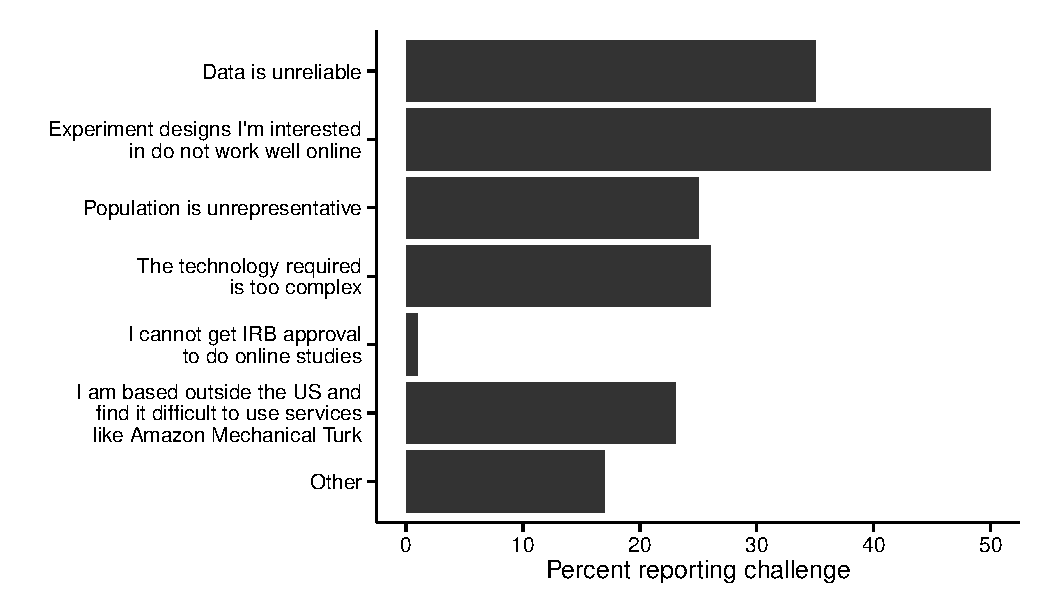
\includegraphics[scale=.75]{figures/challenges.pdf}
%\caption{Survey responses in answer to the question ``What are the major challenges 
% in using behavioral data collected online in research?'' \hl{I suggest making this a full page 
% info graphic type thing that shows more of the interesting things in the survey that we 
% can use to open discussion of psiturk's features}}
%\label{fig:challenges}
%\end{figure*}

Respondents also felt that online data collected presented a set of unique challenges 
(Figure~\ref{fig:survey}).  Some felt that the data collected online was unreliable, or the
population unrepresentative. Many expressed that the experiment designs they were interested in did
not work well online, or that web technology is too complex. Researchers based
outside the US reported difficulty using services like Amazon Mechanical Turk.

\begin{table*}[tp]
\centering
\caption{Features the surveyed researchers desire in a software system for online data collection.}
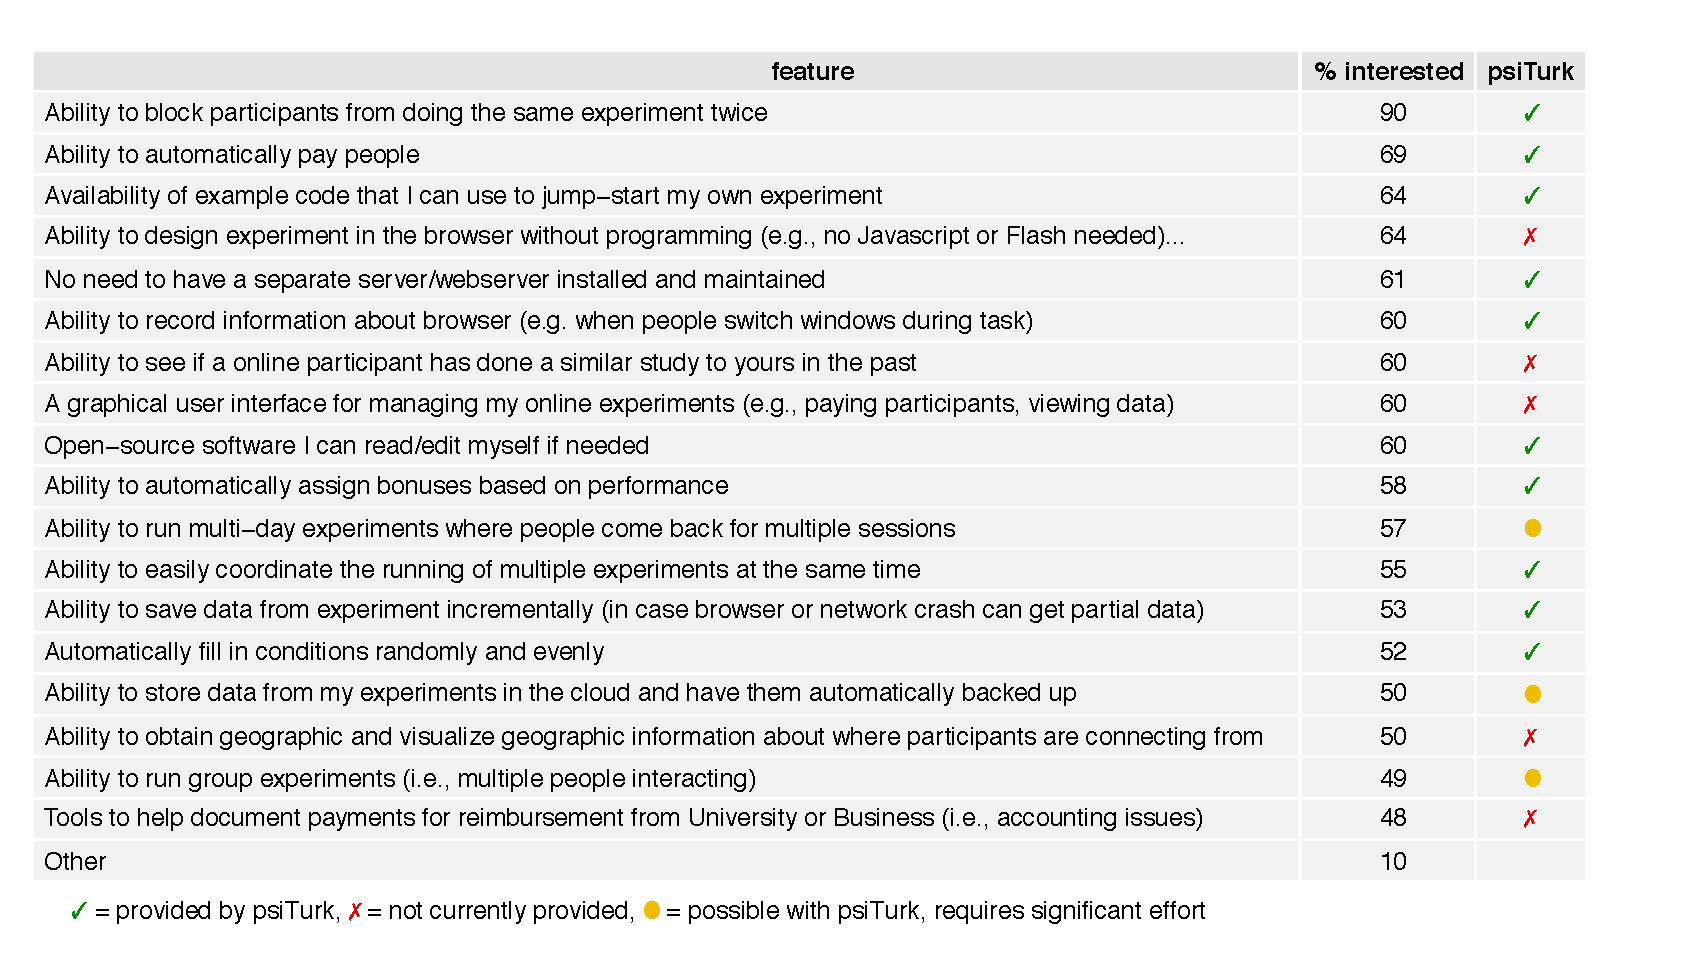
\includegraphics[width=\textwidth]{figures/featuresTable.pdf}
\label{tab:features}
\end{table*}

Many respondents (56\%) listed the tool that they were currently most likely to use as Qualtrics, which is a service for conducting online surveys. However, a majority of participants (79\%) expressed interest in 
being able to run full experiments that included multiple trials which were timed precisely, 
measured reaction time, and other features typical of laboratory studies
(Figure~\ref{fig:survey}). The vast majority (94\%) reported interest in new tools that 
simplified online data collection. A full list of the features researchers were looking for in a 
online data-collection system are shown in Table~\ref{tab:features}, along with a checklist 
showing which are currently handled by \psiturk{}.  Importantly, \psiturk{} successfully
meets many of the major challenges that researchers identified.


\section{\psiturk{} and Amazon Mechanical Turk} 

\psiturk{} was primarily designed to facilitate online data collection using
the Amazon Mechanical Turk (AMT) crowdsourcing platform, though it can also be
used to run experiments in a traditional lab setting.
\cite{Mason:2012xy} provide a general overview of AMT features of
interest to academic researchers, one of which is that it provides a way for researchers
to easily recruit and compensate individuals for online experiments.  
People who complete tasks (called \emph{Human Intelligence Tasks} or \emph{HITs}) are 
called \emph{workers}, and people who post tasks are called \emph{requesters}.
Beyond providing a platform to connect requesters and workers, AMT places few restrictions 
on the type of work that can be requested.  Workers are 
paid a fixed amount for each HIT they complete; this amount is determined by the requester and
can be supplemented with bonus payments for good performance.

From a worker's perspective, the AMT website provides an up-to-date listing of HITs that 
are available, with a title, brief description, and payment amount.  A worker can click on a HIT to 
see its full \emph{advertisement} (an embedded webpage that is either hosted by
Amazon or the requester) and decide to accept the HIT. Once the HIT has been accepted,
the worker must complete it within a timeframe specified by the requester, or \emph{return} the HIT
so that it may be completed by a different worker. The HIT may be completed either 
on a requester's own hosted service (i.e., a webpage 
external to the AMT site), or on the AMT website itself through the use of customized templates.
Upon completion, the worker \emph{submits} the HIT, after which point the completed work must 
be approved by the requester before they are compensated.
In addition, some HITs offer bonus payments that are determined by the requester based 
on a worker's performance.

From a requester's perspective, AMT provides a web-based interface for creating/managing 
HITs and approving work that has been submitted.  In addition, it offers a \emph{sandbox} version 
of the platform in which HITs can be tested without paying live participants.
For basic tasks like surveys and open text fields, AMT offers a range of built-in templates that 
can be used to create experiments within the AMT website.  However, the degree of customization 
is limited for these templates. In particular, they do not support advanced experimental logic that is 
common to many psychology experiments (e.g., adapting the presentation of stimuli based on 
performance, or counterbalancing across a number of experimental variables).
In addition, they are limited to relatively simple forms of interaction and stimulus presentation.

For more complex tasks, a requester can provide a link to their own hosted web page or
web application. This \emph{external HIT} only interfaces with AMT at the beginning of the task (receiving 
basic information about the worker) and at the end of the task (sending confirmation that the task 
has been completed); the requester's web application is responsible for otherwise running the 
experiment and saving the data.  Thus, external HITs enable a much wider range of experiments at 
the cost of additional technical requirements.
% Specifically, it allows you to:
% 1. Run a web server for your experiment
% 2. Test your experiment
% 3. Interact with AMT to recruit, post HITs, filter, and pay participants (AMT workers)
% 4. Manage databases and export data



\section{What technical challenges is \psiturk{} designed to solve?}

The \psiturk{} platform is designed to handle many of the requirements associated with online experimentation---in particular, external HITs on Amazon Mechanical Turk---so that researchers can run complex and sophisticated experiments more efficiently.

\subsubsection{Web server and database management}
\label{sec:web-and-database}

To collect experimental data on the web, or specifically to run an external HIT on AMT, 
researchers minimally need a web server and database.  
The role of a web server is to respond to requests from participant's Internet browser 
for the experiment content.  The role of the database is to save the data provided by 
the participant.  Although less common in laboratory experiments, databases are 
necessary for online studies because it is impossible to save data to a participant's 
computer using a web page or web application -- data must be stored on the server,
rather than the client.  In addition, multiple participants often complete an 
experiment concurrently which can result in file corruption if two people try to
write to the same file at the same time. Databases are specifically designed to 
mitigate this issue by managing concurrent reading and writing.
 
Setting up a web server and database can be complex.  Some universities and colleges
provide these types of services, but the technical infrastructure at other 
institutions is lacking.  \psiturk{} includes a custom webserver and database
as a basic feature of the software tool which can be run from any computer
including a standard office computer or laptop.  This allows data collection from
anywhere without the need for a dedicated server computer.  In addition, \psiturk{}
can be installed on free hosting services such as Amazon Web Services
or RedHat's OpenShift.  Data collected with \psiturk{} is stored at a location
chosen by the experimenter and never visible to the \textsf{psiturk.org} cloud
services or Amazon, protecting the privacy of participants and helping with IRB compliance.

An additional complication is that contemporary web browsers are increasingly security
focused.  In particular, certain browsers will not load content that is not properly 
signed with a SSL certificate and accessed with a \textsf{https://} request.  Such certificates
are often difficult to obtain from universities and can be costly from online
hosting companies.  \psiturk{} solves this problem on behalf of researchers by
using a cloud-based \emph{Secure Ad Server} which presents securely signed
content for users.  One way to think of the Secure Ad Server is as a digital
version of a bulletin board which is used to advertise particular
studies within a university.


\subsubsection{Communicating with AMT}

When using AMT to recruit and compensate participants,
experimenters typically use the AMT website.  This often
involves a lot of manual, error-prone clicking.  To mitigate this, \psiturk{}
has scripted many of the common
tasks that researchers have to do on AMT's website, including:
paying all participants, assigning bonus payments, checking the current
account balance, and monitoring the progress of an experiment.
These tasks are performed via an interactive UNIX-based command
line tool, which helps to prevent errors in payments and
by saving researchers considerable time.

\subsubsection{Programming an experiment}
\psiturk{} provides a number of features which help researchers implement 
experiments.  These include a JavaScript library (\psiturkjs{}), basic HTML templates 
for commonly used components (e.g., consent forms and instruction screens), 
and a user-contributed \emph{Experiment Exchange} where researchers can share the code for their \psiturk{}-compatible
projects (\textsf{http://psiturk.org/ee}). 

The \psiturkjs{} JavaScript library provides basic functions for recording data and sending it back to the \psiturk{} server,
preloading pages and images, as well as some basic functions for looping through instructions
screens and providing (and recording) informed consent.
However, the \psiturk{} framework is \emph{not} designed as a generic
programming interface for building 
experiments (e.g., it does not provide code for widgets such as sliders or buttons) and assume
researchers will use some basic JavaScript, HTML, and CSS to design their experiment.  \psiturk{}'s
philosophy is that general purpose JavaScript libraries available online for creating dynamic content (e.g., jQuery or
Twitter's Bootstrap library) provide the most powerful and well-documented set of features.  

Rather than reimplenting the functionality of existing libraries, \psiturk{} aims to help share code and propagate ``best practices'' among the research community.
These goals are supported by the online Experiment Exchange, which catalogues existing \psiturk{} experiments. The source code for projects in the exchange can be downloaded and modified for a new use,
replicated directly, or can simply provide example of code implementing a particular 
feature.  In addition to the exchange, \psiturk{} also includes a complete working example 
experiment that can be used as a template for new projects.

%That is, it requires that the experimenter knows some basic JavasScipt, HTML, and CSS to code the logic and looks of a new study.


\subsubsection{Recruiting, filtering, and instructing participants}
Finally, \psiturk{} has a number of features for controlling the recruitment
of participants which can contribute to higher quality control.
For example, \psiturk{} offers basic capabilities for assigning workers to different experimental conditions 
and counterbalancing different aspects of the experiment.
In addition, it allows experimenters to filter workers in particular ways.  For example, through \psiturk{},
is it possible to exclude participation by workers using certain devices (such as phones or tablets) or browsers
which are known to have compatibility issues with the experimenter's design (for example,
Firefox or Internet Explorer).  \psiturk{} also allows researchers to prevent a worker from 
participating in the same experiment more than once (which might otherwise be tempting when
large financial rewards are offered).  Future versions of \psiturk{} may also allow researchers to 
block AMT workers who have completed certain \psiturk{} experiments in the past, such as
any experiment with a similar task~\citep[see][for a discussion about non-naivety amongst AMT workers]{chandler2014nonnaivete}.

\begin{figure*}[tp]
\centering
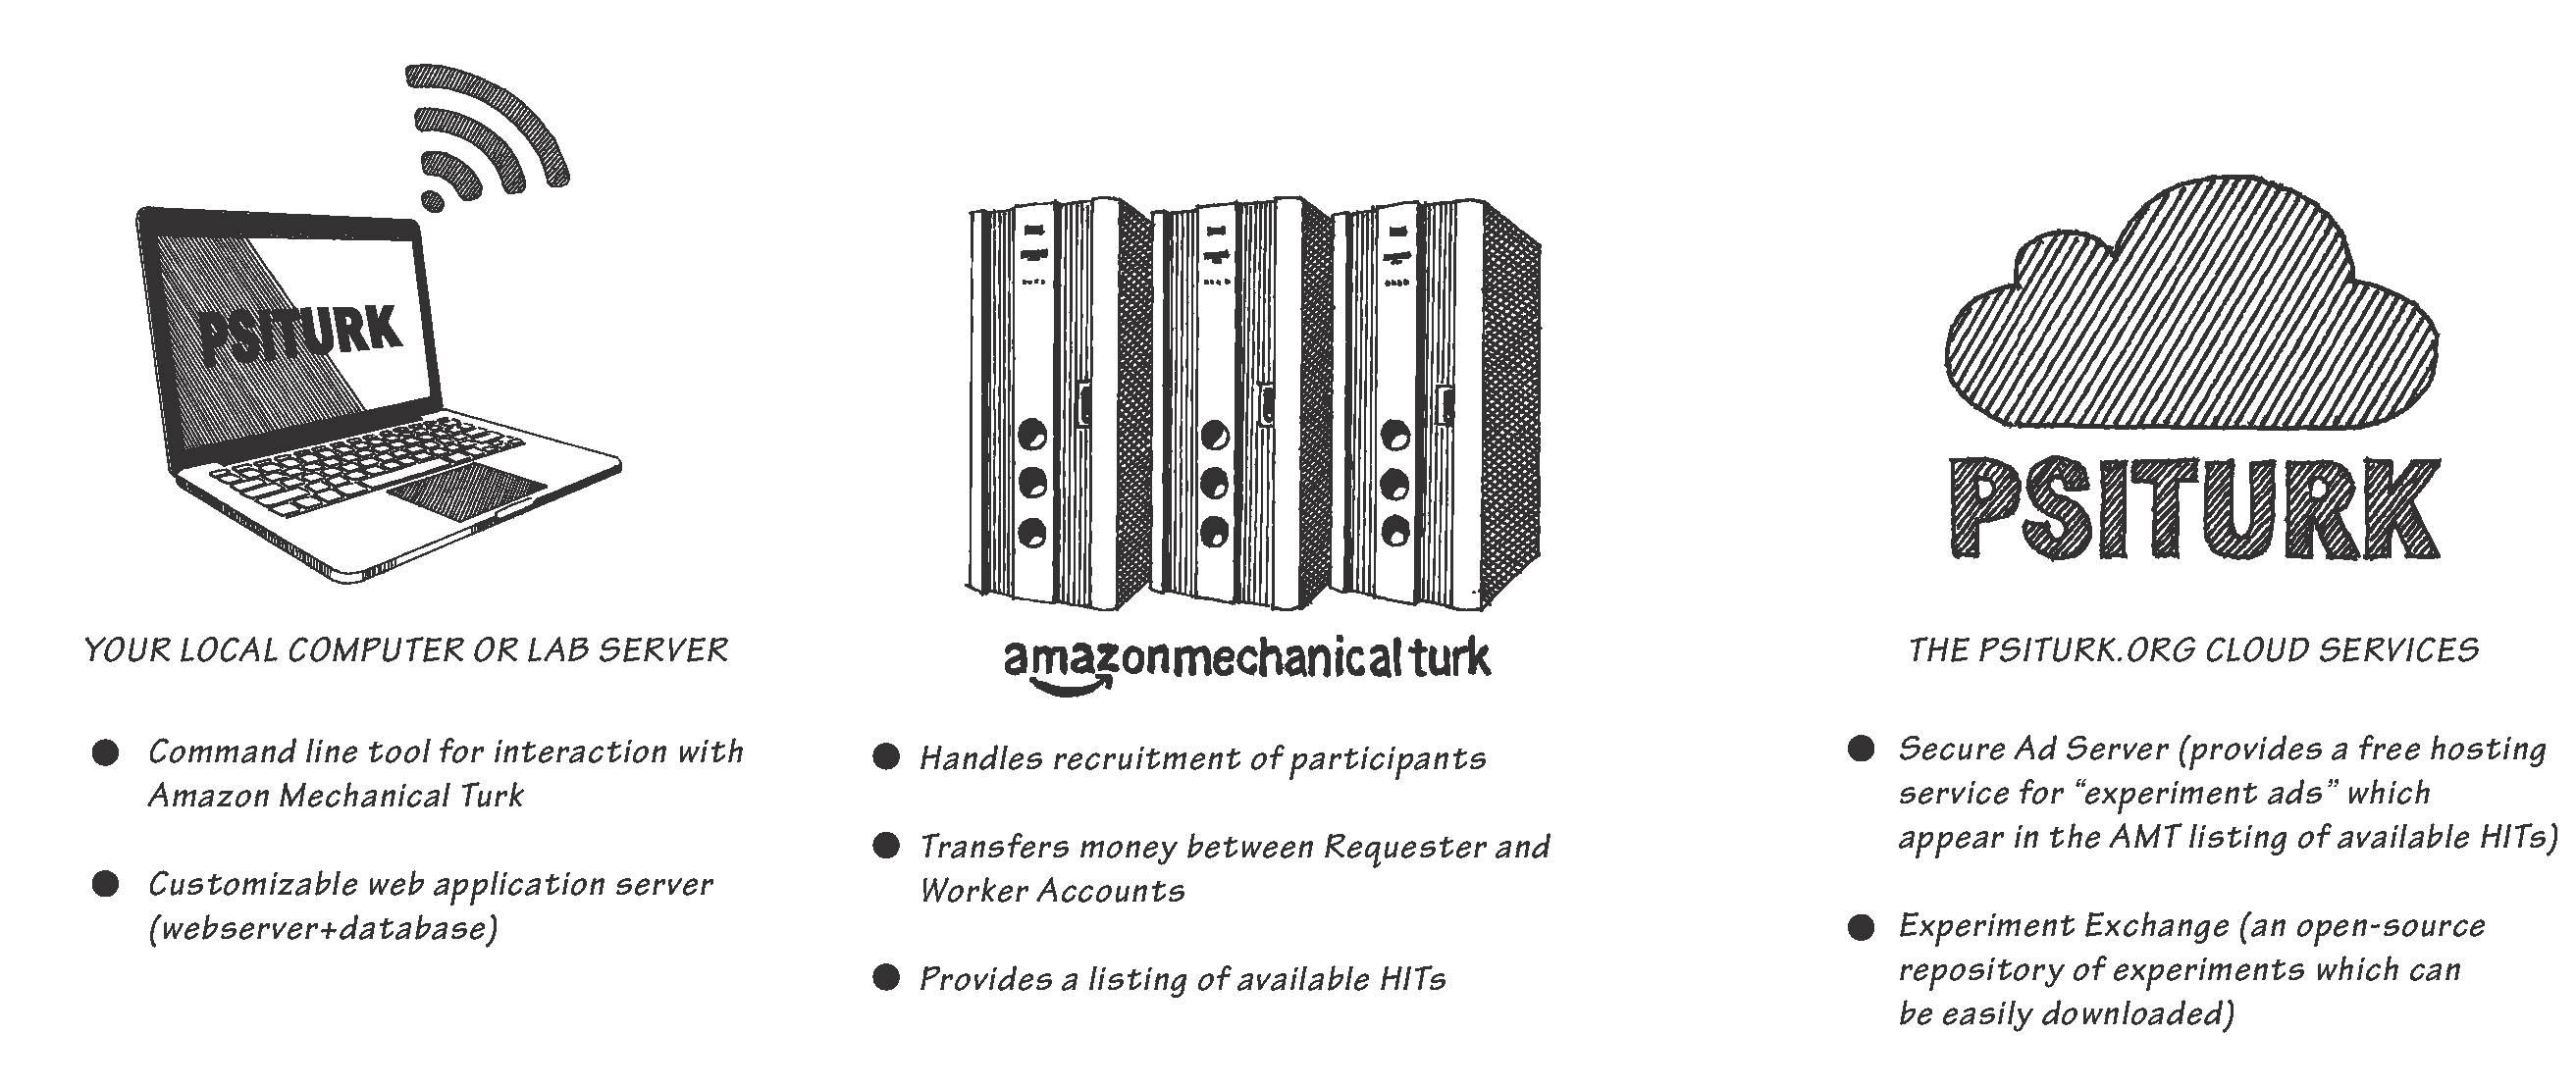
\includegraphics[scale=.40]{figures/psiturk-components.pdf}
\caption{The three core components of the \psiturk{} system.  }
\label{fig:components}
\end{figure*}


\section{Key components of the \psiturk{} platform}

In the last section, we described the technical challenges that \psiturk{} was designed to address. Now, we describe how these challenges are actually met by giving a more detailed overview \psiturk{}'s different components.

The overall structure of \psiturk{} is shown in Figure~\ref{fig:components}
and can be conceptualized as involving three components.
First, there are a collection of software tools which run locally on a user's
 computer or server.  These local components include a command line tool and 
a web application server (which provides both a customizable webserver and 
database solution).  Second, \psiturk{} relies currently on Amazon
Mechanical Turk to handle the recruitment and compensation of participants.
Third, the \textsf{psiturk.org} cloud based component includes a hosted \emph{Secure Ad Server}
and the \emph{Experiment Exchange}.  In the following sections we highlight the important 
functions of each component.

\subsection{Local computer or server}

\subsubsection{Command line tool}
\label{sec:cli}

When using \psiturk{}, the researcher runs an
interactive UNIX-based command line interface (CLI) on a local computer, such as a laptop
or lab computer. This tool is used to issue commands, and to interact with the
Amazon Mechanical Turk system and with the \psiturk{} cloud.  Example
uses of the command line tool include checking the user's Amazon Mechanical
Turk account balance, paying participants, and creating new HITs. In addition,
the command line has the capability to give automated bonus payments to
participants based on a function designed by the experimenter. This feature is
particularly helpful since the AMT website requires bonuses to be entered by
hand for each participant individually.

There are several advantages to designing \psiturk{} as a simple CLI beyond its
efficiency of use. This design makes the user interface code clear and easy to
read and write, allowing newcomers to quickly understand and contribute to the
open-source project. Integrating a new feature into the interface is as simple
as describing the syntax and functioning of a new command; in contrast to a
graphical user interfac (GUI), extending the CLI does not require designing
time-consuming GUI elements.  The CLI also ensures that \psiturk{} is easy to
interact with not just on a laptop or desktop, but also on a remote server or
in the cloud, where users may only have terminal access.


\subsubsection{Web application server (webserver + database)}

The command line tool is also used to interact with the web application server.
The web application server handles the logic determining which pages to show
to a participant at different stages of the experiment.  \psiturk{} comes with
a default web application which implements many important features commonly
needed by experiments (e.g., checking that a user hasn't already done the experiment,
recording and saving data to a centralized database).  In addition, the web application itself
server can be heavily customized to support functions that are difficult to code in JavaScript,
or easily exploitable by savvy participants. Such customizations might be as simple as changing
the way that bonuses are assigned to participants, but they can also allow for much
more complex experimental designs. For example, \psiturk{} allowed us to create an
experiment where a cognitive model is fit to participant's data in real time and used to determine the sequence of future
trials in the experiment.

\subsection{Amazon Mechanical Turk and Amazon Web Services}

Amazon Mechanical Turk's servers handle the recruitment of participants via
its crowdsourced labor force.  It also handles the transfers of money between Requesters and
Workers.  Finally, it provides a listing of available HITs which workers can browse 
through.  Amazon Mechanical Turk is one part of a larger collection
of cloud-based services provided by Amazon via the Amazon Web Services.
For example, by using the \psiturk{} command line tool, users can create a
database server running on Amazon's cloud with a few short commands.  This database
can then be used instead of a local database solution.

\subsection{\textsf{psiturk.org} cloud services}
In addition to the command-line tool and the web application server, \psiturk{}
provides a few web services that are continuously running on a separate web server.
Most important of these is the \psiturk{} Secure Ad Server.  As mentioned earlier, when an experimenter
creates a new HIT and posts it to AMT, they need to display an \emph{ad} explaining how long the task will take and how
much it will pay.  However, ads will not correctly display
in workers' browsers unless they are encrypted using SSL.  To resolve this issue, the
Secure Ad Servier allows users of the \psiturk{} system to host ads on the \textsf{psiturk.org}
website which are encrypted.

Besides the convenience of the Secure Ad Server in terms of providing
SSL signed URLs, the Secure Ad Server tracks statistics about the
number of workers who viewed the ad but decided to not accept it, the
number who accepted it, and the number who actually completed the task.
These statistics are made available on the \textsf{psiturk.org} dashboard
and can be an additional source of information for experimenters.

Finally, in addition to the Secure Ad Server, the \psiturk{} Experiment Exchange provides
a open-source repository of \psiturk{}-compatible experiments which can be 
easily downloaded.  The coordination of these downloads is handled by the \textsf{psiturk.org} cloud. 

%Complete documentation and tutorials are available at http://psiturk.org/docs, including instructions for installing the software.

\section{Requirements and initial setup}
This section describes the requirements and installation steps that are required to successfully setup \psiturk{} and run
HITs on Mechanical Turk. Note that details of these steps may change over time and will be updated at \textsf{http://psiturk.readthedocs.org}.

\subsection{System requirements}
\psiturk{} is designed to run on UNIX systems (including Mac OS X, BSD, and Linux) that satisfy the following requirements:

\begin{enumerate}
\item A working installation of Python 2.7 (Python 3 is not currently supported)
\item The \texttt{pip} package manager 
\item A command line tool (like \emph{Terminal} in Mac OS X)
\item A web browser (ideally one that provides web developer tools, like Firefox, Safari, or Chrome)
\end{enumerate}

To satisfy the Python requirements, we recommend using an existing distribution like \emph{Enthought} or \emph{Anaconda}. These are free
Python distributions that ship with a range of useful packages, including the \texttt{pip} package manager. 

\subsection{AWS credentials}
An Amazon Web Services (AWS) account is required to use AMT as a requester. A new account can be created at \textsf{http://aws.amazon.com/mturk/}. 
To set up an account, note that requesters
must provide a U.S. billing address, so this may bar researchers outside the U.S. from creating an account. 

After setting up an account, \psiturk{} users must retrieve their AWS credentials, which include an \emph{access key id} and a
\emph{secret access key}. These can be retrieved and (re-)generated at \textsf{https://console.aws.amazon.com}.
Eventually, these credentials will be entered in the \texttt{.psiturkconfig} file, as explained below.


\subsection{\psiturk{} credentials}
Additionally, a \psiturk{} account must be created at \textsf{https://psiturk.org/register}, which allows users to 
post ads on \psiturk{}'s Secure Ad Server. A new user must then obtain a set of \psiturk{} credentials which can be found in 
the ``API Keys'' menu item in the drop-down at the top right hand of the page.
These credentials will also be placed in \texttt{.psiturkconfig} (see below).

\subsection{Installation}
\psiturk{} is installed using the python package manager \texttt{pip}. In a terminal window, type\footnote{Depending on the user's permissions, this command may have to be prefaced with \texttt{sudo}.} (excluding the dollar sign):

\begin{lstlisting}
$ pip install psiturk
\end{lstlisting}

Alternatively, \psiturk{} can be installed directly from GitHub, which holds the latest stable
release in the \texttt{master} branch, and the latest development version in the \texttt{dev} branch. 
To install from \texttt{master}, for example, type:

\begin{lstlisting}
$ pip install git+git://github.com/NYUCCL/psiTurk.git@master
\end{lstlisting}

The \psiturk{} installation automatically creates a global config file, \texttt{.psiturkconfig}, in a user's home directory. 
This file must then be edited to include the AWS and \psiturk{} credentials of the specific user. 

\subsection{Optional: Adding a SQL database}
By default, \psiturk{} includes a basic database solution called \emph{SQLite}. This solution
will work for HITs that only require light traffic, but it does not handle
multiple concurrent queries well: there is a danger of data loss when a SQLite database is 
accessed at the same time by different users. 
It is therefore recommended to set up a more robust database solution, like a
MySQL database, especially if a researcher wants to run many participants simultaneously.
Fortunately, Amazon's Web Services (of which Mechanical Turk is just one component)
provides a relatively simple and inexpensive way to set up a SQL server.  Please refer to
the documentation at \textsf{http://psiturk.readthedocs.org/} (``Configuring Databases'' section)
for complete instructions.

\section{Getting started with \psiturk{}}

The following section provides a basic overview of how to use \psiturk{},
explaining the various steps required of new users of the system along with
some details about how the various components described above interact.

\subsection{Configuration and project structure}

A new \psiturk{} project can be initialized in the current directory using (without the dollar sign):

\begin{lstlisting}
$ psiturk-setup-example
\end{lstlisting}

\noindent This creates a new directory containing an example experiment,
which can be used as a template for more sophisticated designs.
The project directory typically includes the following files (though some are only
created after the experiment is run for the first time):

\begin{itemize}
\item \texttt{config.txt}: a text file containing settings for the current experiment, including:

\begin{itemize}
\item Metadata about the experiment that is displayed to workers on the AMT website (title, description, etc.)
\item Restrictions on which workers can accept the HIT, including geographic location (e.g., limiting to US workers only), AMT-specific qualifications (e.g., a worker's proportion of past work that has been approved), and web browsers that are permitted.
\item Database information (SQLite, by default)
\item Server parameters (URL, port number)
\item Task parameters (e.g., number of conditions)
\end{itemize}


\item \texttt{custom.py}: a Python file containing user-provided custom functionality for the \psiturk{} web server

\item \texttt{participants.db}: the SQLite database (if SQLite is being used)

\item \texttt{server.log}: a log of any messages from the experiment server (\emph{not} from the actual experiment code)

\item \texttt{static/} a directory containing experiment files, including JavaScript, CSS, and images.

\item \texttt{templates/} a directory containing HTML files associated with the experiment 
\end{itemize}

Setting up a new experiment thus entails 1) editing the settings in \texttt{config.txt}, and 2) modifying the contents of the \texttt{static} and \texttt{templates} directories to reflect your experimental design (note that programming the experiment requires at least some basic web programming skills, including HTML, CSS, and JavaScript).

The remaining files are only necessary in order to debug server errors (\texttt{server.log}), add new server-side functionality (\texttt{custom.py}), or to access saved data (\texttt{participants.db}).

\subsection{Command line interface: Managing HITs and serving the experiment}

As described in Section~\ref{sec:cli}, \psiturk{} runs as a command line interface
(CLI) within a standard terminal window and can be used to perform a wide
variety of tasks---from creating HITs and paying workers, to launching Amazon
Web Services database instances, to opening an experiment in a browser for
debugging---that would otherwise be spread across a number of websites and
programs. In most cases, a user of the \psiturk{} CLI will never have to log into
the MTurk website except to add money to their MTurk requester account and
to first create the account (and to accept the terms of service).

Entering
\texttt{psiturk} at the command line in any directory containing a \psiturk{} project launches the
\psiturk{} CLI, which features a colorized prompt that provides important information at a glance, including
whether the server is running, the current mode (\emph{live} or \emph{sandbox}), and the number of HITs currently running on AMT in the same mode:

\begin{lstlisting}
[psiTurk server:off mode:sdbx #HITs:0]$
\end{lstlisting}

\noindent In some examples below, this prompt is truncated as \texttt{[psiTurk]\$} to indicate commands that occur within the \psiturk{} CLI, while commands that are entered at the user's standard command line are preceded simply by \texttt{\$}.

\subsubsection{Example CLI usage}
Commands are organized into groups based on their function, following a general \texttt{command subcommand
arguments} format. For example, one can create a HIT by typing: 

% \noindent\lstinline+[psiTurk]$ hit create+
% $<\# assignments> <\$ amount> <duration>$
\begin{lstlisting}
[psiTurk]$ hit create
\end{lstlisting}

\noindent which launches an interactive prompt for number of assignments, payment per HIT, and HIT duration. The sandbox mode is active by default, which means that calling \texttt{hit create} will submit a HIT to the AMT sandbox website.

After creating one or more HITs, one can list any active HITs with:

\begin{lstlisting}
[psiTurk]$ hit list --active
\end{lstlisting}

The experiment server is launched using:

\begin{lstlisting}
[psiTurk]$ server on
\end{lstlisting}

\noindent which opens the port specified in the project configuration file, \texttt{config.txt}.
The experiment server will then respond to incoming requests, assuming that the port is publicly accessible.
This requires a static IP to prevent the experiment's URL from changing.
Users without a static IP address can use a dynamic DNS service to forward requests to their dynamic IP.
If the system running \psiturk{} is behind a router, the router must be configured to forward requests on the same port.

During the development of an experiment, the current code can be tested using:

\begin{lstlisting}
[psiTurk]$ debug
\end{lstlisting}

\noindent which will open a new browser window in which the current experiment can be tested. The experimenter can then test the experiment from the perspective of a worker before making it publicly available.
Once the experiment is ready for real workers, the \texttt{mode} command can be used to switch to \emph{live} mode, after which newly created HITs will be submitted to the main AMT site.

Help on any of the commands is easily accessible through the \texttt{help} command. Using \texttt{help} on its own will print all available commands, and using \texttt{help command} will print out detailed help on the given command.

\begin{figure*}[tp]
\centering
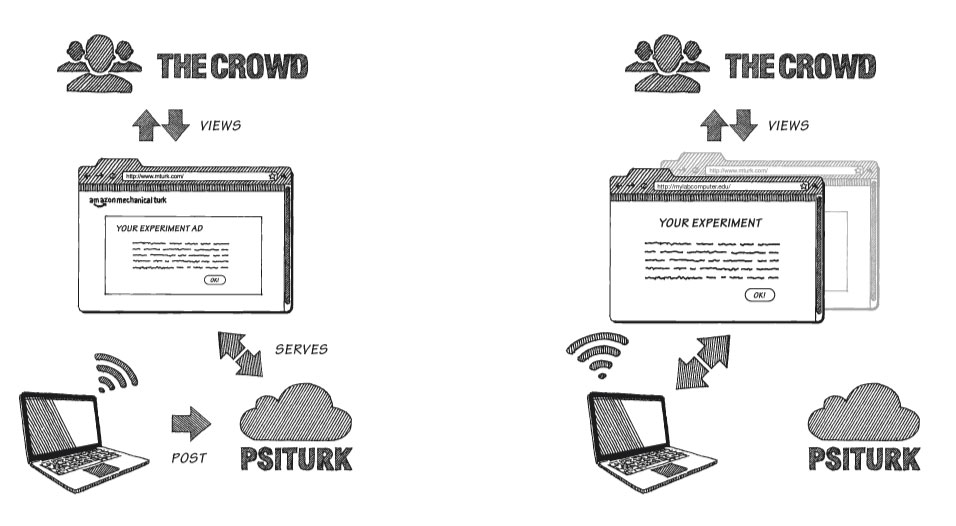
\includegraphics[scale=.40]{figures/psiturk_cloud_sequence.jpg}
\caption{How the Secure Ad Server works.}
\label{fig:adserver}
\end{figure*}


\subsection{The Secure Ad Server}
\label{sec:adserver}

As described briefly in Section~\ref{sec:web-and-database}, the \textsf{psiturk.org}
cloud service provides a \emph{Secure Ad Server}.  The term \emph{ad} in this context
refers to a small HTML page which describes the details and requirements of a
given experiment.  The ad is the first interaction that an experimenter has
with a potential subject and is thus the gateway to subject recruitment. Ads
are in many ways analogous to hanging a poster or flyer around a university
building in order to recruit participants. It's easy to overlook the importance
of a good ad, and making that ad visible to as many participants as possible.

An overview of the flow of running an experiment using
\psiturk{} and the Secure Ad Server is illustrated in
Figure~\ref{fig:adserver}.  When a researcher using \psiturk{}
runs the \texttt{hit create} command, the current contents of the local
\texttt{templates/ad.html} file are uploaded to the \textsf{psiturk.org} cloud (see
the right panel of Figure~\ref{fig:adserver}).
This will create a unique custom URL for the experiment (an example might be
\textsf{https://ad.psiturk.org/view/90812390123091823}) which
allows anyone on the internet to view the contents of the uploaded \texttt{ad.html}
file.  Critically, the ad URL is encrypted and
securely signed with an appropriate SSL certificate ensuring that all
web browsers will successfully display the webpage\footnote{SSL certification has recently become a requirement for hosting content within an \texttt{iframe} on \texttt{mturk.com}.}. A different URL is created each time \texttt{hit create}
is run and there is no limit to the number of ads that can be created.  A private listing of all ads created by a particular user is available on the \textsf{psiturk.org} dashboard (\textsf{https://psiturk.org/dashboard}).

The custom ad URL is automatically passed
on to AMT by the \texttt{hit create} command as the location of
the selected HIT.  As is visible in Figure~\ref{fig:adserver},
when an AMT worker views a HIT on the AMT
website, it loads the ad from the \textsf{psiturk.org} cloud server (left panel of Figure~\ref{fig:adserver}).  If the worker accepts
the hit, a link is provided to the worker which pops open a new browser
window.  This URL points directly at the location of the \emph{requester's} local computer
or server (right panel).  After this hand-off occurs, all data is transmitted directly between the worker
and the requester: the \textsf{psiturk.org} cloud server does not ever
process or see the user's experimental data.  This is important for many IRBs,
particularly if an experiment involves sensitive materials.


\subsection{JavaScript library \psiturkjs{}}

The JavaScript library \psiturkjs{} enables interaction with the server from the client-side (JavaScript) experiment code.
The goal of the library is to handle the most common functionality of \psiturk{}-based web experiments, without imposing any additional requirements on the structure or design of the experiments themselves.
Researchers can use any third-party JavaScript libraries to design their experiment, while relying on \psiturkjs{} for common functions, including saving data and notifying the server of changes in a participant's status.

Listing~\ref{code.lst} shows a condensed version of the JavaScript code from the Stroop example experiment.
This is used in the following sections to illustrate how experiment code uses functions from \psiturkjs{} in order to interact with the \psiturk{} server.
For the full, functional version, see the file \texttt{static/js/task.js} in the example experiment directory.

\subsubsection{Initialization}

When the experiment files are requested from the \psiturk{} server, the following global variables are also set (see \texttt{templates/exp.html}):

\begin{itemize}
\item \texttt{uniqueId}: a unique identifier for the participant
\item \texttt{adServerLoc}: the experiment-specific URL on the Secure Ad Server
\item \texttt{mode}: the current mode (debug, sandbox, or live)
\item \texttt{condition}: experimental condition
\item \texttt{counterbalance}: counterbalancing code, used to vary design elements that are not related to main manipulation 
\end{itemize}

A \texttt{psiTurk} object must be initialized based on these global variables (line 2).
These variables can also be used to change the experimental logic.
For example, a common requirement is to change the stimulus set or design based on the condition or counterbalance codes that have been assigned by the \psiturk{} server (lines 4-5).

Following instantiation, the \texttt{psiTurk} object can be used to preload a list of HTML pages that reside in the \texttt{templates} directory of the experiment (lines 8-9).
This allows a new page to be displayed using a single command (line 34), which replaces the body of the window with the content in the specified HTML file.
The \texttt{psiTurk} object also has functions for preloading images (in order to avoid server requests in the middle of the experiment when an image is displayed) and a basic structure for presenting a series of HTML pages (e.g., for an instructional phase).

\subsubsection{Tracking a participant's progress in an experiment} 

\psiturk{} records changes in a participant's status as they move through an experiment. 
Some of these status changes are automatic, e.g., when a participant is assigned to a condition or if they quit an experiment early. 
Two additional status changes are initiated by the client-side experiment code using \psiturkjs{} functions.
First, since experiments typically begin with an instructional phase, calling the function \texttt{psiTurk.finishInstructions()} upon completion of this phase will save the participant's status as having begun the main experiment.
If the participant attempts to quit the experiment after that point, they will receive a warning that they will not be able to restart the experiment and may forgo payment.
Second, successful completion of the experiment is signaled by calling \texttt{psiTurk.completeHIT()}, which closes the experiment and redirects the participant to the AMT page to submit their HIT.

\subsubsection{Saving experimental data} 

The experimenter can save data in two formats.
\texttt{psiTurk.recordTrialData} takes any JSON object as input and appends it to a list of \emph{trial data}.
This data structure is meant for sequential data that may be collected over the course of multiple trials or blocks, where each line corresponds to a new measurement.
However, the format of each entry is defined by the experimenter and is saved in the database as a single JSON object (see line 20).
Each new entry is automatically time-stamped at the time that \texttt{psiTurk.recordTrialData} is called.

In contrast, \texttt{psiTurk.recordUnstructuredData} is used to record $(key, value)$ pairs, where the key is uniquely defined within the experiment (see line 43).
This format is useful for survey questions, randomly generated experiment parameters, or other one-time measurements, e.g., (\emph{Age}: 24).

Importantly, both functions above simply record the data in the appropriate format on the client-side (i.e., within the \texttt{psiTurk} JavaScript object).
When the experimenter wishes to save the data to the server they call \texttt{psiTurk.saveData()}, at which point both sets of data are sent to the server to be recorded in the database.
\texttt{psiTurk.saveData()} can also be called with functions that will be executed upon either success or failure of the server request.
For example, if the final save request is successful, the experiment can be terminated with \texttt{psiTurk.completeHIT()} passed as a callback (see lines 56-63).  

\subsubsection{Automatic recording of browser interactions}
 
One general limitation of web experiments is greater uncertainty about a participant's testing environment and engagement with the experiment.
Unlike lab computers where most undesired behaviors can be prevented, a web participant is always able to close a web browser, switch to different applications, or change other aspects of their experience.
However, standard methods exist for recording a user's interaction with a web browser, and this data can be useful for 1) tracking how an experiment was actually displayed, and 2) the level of a participant's engagement.

For example, although it is possible to control the initial size of a browser window, a web participant can change the dimensions of the window, potentially obscuring or altering the displayed elements.
\psiturkjs{} automatically records these changes in the size of the window.
Similarly, the participant can choose to switch focus away from the experiment window (e.g., to another browser window or a different application).
\psiturkjs{} automatically records every time that the experiment window loses and gains the participant's focus.
This \emph{event data} is saved to the database whenever \texttt{psiTurk.saveData} is invoked, without any additional action on the part of the experimenter. \\


\begin{lstlisting}[float=*,numbers=left,numberstyle=\small\color{gray},caption=Condensed version of JavaScript code for Stroop experiment,label=code.lst]
// Initalize psiturk object with parameters passed from server (see templates/exp.html)
var psiTurk = new PsiTurk(uniqueId, adServerLoc, mode);

var mycondition = condition;  // these two variables are passed by the psiturk server process
var mycounterbalance = counterbalance;  // they tell you which condition you have been assigned to

// All HTML snippets to be loaded from templates directory
var pages = ["instructions/instruct-1.html", ...];
psiTurk.preloadPages(pages);

var StroopExperiment = function() {
	...	
	var response_handler = function(e) {
		...
		if (response.length>0) {
			listening = false;
			var hit = response == stim[1];
			var rt = new Date().getTime() - wordon;

			psiTurk.recordTrialData({'phase':"TEST",
                                     'word':stim[0],
                                     'color':stim[1],
                                     'relation':stim[2],
                                     'response':response,
                                     'hit':hit,
                                     'rt':rt}
                                   );
			remove_word();
			next();
		}
	};
	...	
	// Load the stage.html snippet into the body of the page
	psiTurk.showPage('stage.html');
	...
};

var Questionnaire = function() {
	...
	record_responses = function() {
		psiTurk.recordTrialData({'phase':'postquestionnaire', 'status':'submit'});
		$('textarea').each( function(i, val) {
			psiTurk.recordUnstructuredData(this.id, this.value);
		});
		$('select').each( function(i, val) {
			psiTurk.recordUnstructuredData(this.id, this.value);		
		});
	};
	... 
	// Load the questionnaire snippet 
	psiTurk.showPage('postquestionnaire.html');
	psiTurk.recordTrialData({'phase':'postquestionnaire', 'status':'begin'});
	
	$("#next").click(function () {
		record_responses();	
		psiTurk.saveData({
			success: function(){
			    psiTurk.computeBonus('compute_bonus', function() { 
			    	psiTurk.completeHIT(); // when finished computing bonus, quit
			    }); 
			}, 
			error: prompt_resubmit});
	});
};
\end{lstlisting}

\subsection{Experiment Exchange}

A significant advantage of web-based experiments is the potential for low-friction replication and extension. 
The \emph{Experiment Exchange} (\textsf{https://psiturk.org/ee}) facilitates the sharing of experiments that have been built to run using \psiturk{}, acting as an ``app store'' for \psiturk{}-compatible designs.
Once an experiment has been completed, a researcher can submit the following information to register their experiment on the exchange:

\begin{enumerate}
\item A GitHub repository containing the project code
\item Metadata about the experiment, including a title, description, and keywords
\item The DOI for the paper describing the results of the experiment (if any)
\item The version of \psiturk{} that was used to run the experiment
\end{enumerate}


Metadata associated with an experiment allows other researchers to discover it through the \psiturk{} website.
A publicly available experiment can then be downloaded using the following command in the terminal:

\begin{lstlisting}
$ psiturk-install <experiment-specific-id>
\end{lstlisting}

\noindent with the experiment-specific identifier found on the exchange page.
If \psiturk{} is already configured on the user's system, the downloaded experiment will run without further changes, and can then act as a starting point for direct replication or extensions.
Modified versions can then be re-run using the same population via AMT, thereby minimizing the potential for experimenter-specific biases.

Other initiatives (e.g., the Open Science Framework, \textsf{https://osf.io}) also aim to improve the transparency, reproducibility, and efficiency of research through centralized services, but are less focused on the specific technology stack used to run online experiments.
In contrast, the \psiturk{} Experiment Exchange links together experiments that can be run within a common framework.
As a result, existing experiments can serve as examples to help new researchers learn to code for the web; they shorten the development time necessary (especially for popular experimental paradigms); and the exchange facilitates communication between researchers with similar interests.

\section{Adoption by the community}

At the time of publication of this paper, there are 267 registered users accounts
on \textsf{https://psiturk.org}.  So far 8,432 distinct Amazon workers have completely
\textsf{psiTurk} tasks and 1,788 attempts to complete the same experiment more
than once have been blocked.   The \textsf{psiTurk} command line tool itself has been
launched 20,823 times.  In addition, the source code for six \textsf{psiTurk}-compatible experiments
have been published in the Experiment Exchange including some by researchers
who are not authors of this article.

\section{Limitations and future directions}

\psiturk{} solves a number of the challenges facing researchers interested in online data collection.
However, at the time of the publication of this article, there remain a number of limitations 
that remain to be solved.

One possible limitation is that \psiturk{} is currently designed to work primarily with Amazon Mechanical Turk. 
A common worry with AMT is the unrepresentativeness of its subject pool (in terms of demographics and 
geography), as well as the fact that certain experimental protocols are now too well-known to workers to guarantee naive
participants~\citep{chandler2014nonnaivete}.  Indeed, some of the concerns raised by survey respondents in Section 2 are inherent 
to online data collection or the AMT platform and therefore \psiturk{} does not address them.
It is worth pointing out, however, that the common concern about data reliability may be somewhat exaggerated 
based on recent studies that have successfully replicated a wide range of classic cognitive psychology findings using 
AMT data~\citep{crump2013evaluating}. Interestingly, this study also found that increasing worker payment had no effect on 
reliability, suggesting that even  at low payment levels data quality was high. 

On the other hand, there clearly exist experimental protocols that simply are not amenable to online
experimentation. Experiments that require very fine-grained temporal control over stimulus presentation, for example, 
may be unsuited because browsers will not be able to reliably display content fast enough if the presentation time
becomes too short~\citep{crump2013evaluating}.
Similarly, any experiment that requires control over a participant's screen size, resolution, or distance from the screen will 
be problematic due to the nature of the web browsing environment.
One advantage of \psiturk{} is that it automatically collects data on worker's interaction with the experiment window, that is, 
if and when the window was resized and if and when the user switched tabs or windows. 
This kind of data can be used to evaluate a worker's level of engagement while completing the task.

As a result of these concerns, some experimenters may look for alternatives to AMT. 
Many \psiturk{} features (i.e. the web server, data base, and \psiturkjs{}) are general enough to facilitate running experiments 
on other platforms, too, but it would require some customization of certain AMT-specific functionality. 
Researchers who decide to use \psiturk{} on another platform could contribute such changes to the GitHub repository 
(\textsf{https://github.com/NYUCCL/psiTurk}) to make them available to the community.

Another limitation is that \psiturk{} only runs on UNIX systems, like Linux and Mac OS, and can thus not be used on Windows computers. To meet this 
challenge, one option for Windows users is to use a cloud-based computing service to run \psiturk{} and host experiments. There exist
multiple free or low-cost options, such as Amazon Web Services (\textsf{https://aws.amazon.com}). 
The installation steps and setup may diverge slightly from the standard procedure but  the \psiturk{} documentation already contains 
additional installation instructions for OpenShift. In the future, we hope to extend support  and documentation to a wider range of cloud 
computing options.

Another future direction is to extend the counterbalancing capabilities of \psiturk{}. Currently, the built-in counterbalancing algorithm
simply aims to assign participants equally to different cells.  However, this equal assignment method can be problematic if, for instance, 
one group has a higher drop-out rate than the others (a problem rarely encountered in the lab). 
In that case the high drop-out group will need to receive
more participants to equalize the difference and thus assignment probabilities will no longer be equal across groups. We are
currently working on alternative counterbalancing algorithms that keep assignment probabilities equal (which may then lead to unequal
number of participants) to avoid this problem. 

One exciting prospect of running online experiments is to let multiple participants interact to study coordination
or group behavior. Currently \psiturk{} does not offer its own tool to facilitate such multi-person experiments, but we would like to
add support for it in the future, using web-sockets or other protocols that enable communication between users.

\section{Conclusions}

As online data collection becomes more widespread, new software tools will need to be
created.  While in some cases these tools may come from for-profit enterprises, the project
described in this paper advances an open-source, community-driven approach to software
design.  A core philosophy is that better scientific software developed can be developed 
with more diverse input from many programmers~\citep{Raymond:1999zt}.
The advantages are that the quality of the code can be improved by having many people
read and help catch bugs.  In addition, ``best practices" can be more readily propagated
through the research community through code share such as in the \textsf{psiTurk}
Experiment Exchange. 


% BibTeX users please use one of
\bibliographystyle{spbasic}      % basic style, author-year citations
%\bibliographystyle{spmpsci}      % mathematics and physical sciences
%\bibliographystyle{spphys}       % APS-like style for physics
\bibliography{psiturk}

\end{document}
